\documentclass[titlepage,openright,twoside,a4paper,10pt]{report}

\usepackage[top=3.5cm, left=3cm, right=3cm, bottom=2.5cm]{geometry}
\usepackage[unicode]{hyperref}
\usepackage{fontspec} %if I end up using special font.
\usepackage{csquotes} %something about multilingual quotes.
\usepackage{siunitx}
\usepackage{wrapfig}
\usepackage{footnote}
\usepackage[ruled,vlined,linesnumbered,longend]{algorithm2e} %algorithms?
\usepackage{titlesec}
\usepackage{titletoc}
\usepackage[font={small}]{caption}
\usepackage{subcaption}
\usepackage{fancyhdr}

% My additions
\usepackage[version=4]{mhchem}
% My additions

\usepackage{polyglossia}
\setdefaultlanguage{english}
\setotherlanguage[variant=modern]{greek}
\setmainfont{GFS Didot}

% Citations, glossaries and bookmarks.
\usepackage[toc,nonumberlist,nopostdot,acronyms,automake]{glossaries}
\usepackage[backend=biber,style=ieee]{biblatex} %I added the biber part.
\usepackage{bookmark}

% Color hyperlinks instead of having a box around them
\usepackage{listings}
\usepackage[table,xcdraw]{xcolor}
\usepackage{graphicx}
\usepackage[export]{adjustbox}
\usepackage{tikz}
\usepackage[labelfont=bf]{caption}
\usepackage{float}

% Maths packages
\usepackage{amsmath, amssymb}
\usepackage{mathtools}
\usepackage{nicefrac}
\usepackage{multicol}

\usepackage{cleveref}

% Commands
\newcommand{\paper}[2]{#1 et al. \cite{#2}} %defines citation reference function
\newcommand{\thetitle}{Type my title here.}

% Prevent huge spaces from the twoside option
\raggedbottom

% Colors
\definecolor{dark_grey}{HTML}{303030} %internal link color, change probably

% PDF properties
\hypersetup{
  pdfstartview= {FitH},
  pdfauthor   = {Nikolaos Kasapakis},
  pdftitle    = {\thetitle},
  pdfsubject  = {Bachelor thesis at the Department of Physics of the Aristotle University of Thessaloniki},
  pdfkeywords = {Neuroscience},
  colorlinks  = true, %Colours links instead of ugly boxes
  urlcolor    = blue, %Colour for external hyperlinks
  linkcolor   = dark_grey, %Colour of internal links
  citecolor   = blue, %Colour of citations
  bookmarksnumbered,
}

\addbibresource{references.bib}

\title{\thetitle}
\author{Nikolaos Kasapakis}
\date{}

\makeglossaries
\newacronym{MVPA}{MVPA}{Multi-Variate Pattern Analysis}
\newacronym{UPA}{UPA}{Univariate Pattern Analysis}
\newacronym{SVM}{SVM}{Support Vector Machine}
\newacronym{ROI}{ROI}{Region of Interest}
\newacronym{ROIs}{ROIs}{Regions of Interest}
\newacronym{BOLD}{BOLD}{Blood-Oxygen-Level-Dependent}
\newacronym{HbR}{HbR}{deoxyhemoglobin}
\newacronym{HbT}{HbT}{total hemoglobin}
\newacronym{HbO}{HbO}{Oxyhemoglobin}
\newacronym{Hb}{Hb}{hemoglobin}
\newacronym{OEF}{OEF}{Oxygen Extraction Fraction}
\newacronym{HCP}{HCP}{Human Connectome Project}
\newacronym{WM}{WM}{Working Memory}
\newacronym{ITI}{ITI}{inter-task interval}
\newacronym{CSF}{CSF}{Cerebrospinal Fluid}
\newacronym{RF}{RF}{radio frequency}
\newacronym{CBF}{CBF}{Cerebral Blood Flow}
\newacronym{ASL}{ASL}{Arterial Spin Labeling}
\newacronym{USA}{USA}{United States of America}
\newacronym{T1w}{T1w}{T1-weighted}
\newacronym{T2w}{T2w}{T2-weighted}
\newacronym{MZ}{MZ}{monozygotic}
\newacronym{DZ}{DZ}{dizygotic}
\newacronym{IQ}{IQ}{intelligence quotient}
\newacronym{T-MEG}{T-MEG}{task-evoked MEG}
\newacronym{EV}{EV}{explanatory variable}
\newacronym{COPE}{COPE}{contrast of explanatory variables}
\newacronym{SVMs}{SVMs}{Support Vector Machines}
\newacronym{PCA}{PCA}{Principal Component Analysis}
\newacronym{ICA}{ICA}{Independent Component Analysis}
\newacronym{PDF}{PDF}{probability density function}
\newacronym{HRF}{HRF}{Hemodynamic Response Function}
\newacronym{GLM}{GLM}{General Linear Model}
\newacronym{NIfTI}{NIfTI}{Neuroimaging Informatics Technology Initiative}
\newacronym{LR}{LR}{Left to Right}
\newacronym{RL}{RL}{Right to Left}
\newacronym{FEAT}{FEAT}{FMRIB's Expert Analysis Tool}
\newacronym{3D MPRAGE}{3D MPRAGE}{three-dimensional magnetization-prepared rapid gradient-echo imaging}
\newacronym{FOV}{FOV}{Field of View}
\newacronym{BW}{BW}{Bandwidth}
\newacronym{ES}{ES}{Echo Spacing}

% fMRI Acronyms
\newacronym{r-fMRI}{r-fMRI}{resting-state fMRI}
\newacronym{t-fMRI}{t-fMRI}{task-evoked fMRI}
\newacronym{dMRI}{dMRI}{diffusion imaging}
\newacronym{fMRI}{fMRI}{Functional Magnetic Resonance Imaging}
\newacronym{MRI}{MRI}{Magnetic Resonance Imaging}
\newacronym{MR}{MR}{Magnetic Resonance}
\newacronym{NMR}{NMR}{Nuclear Magnetic Resonance}

% Imaging Techniques Acronyms
\newacronym{PET}{PET}{Positron Emission Tomography}
\newacronym{NIRS}{NIRS}{Near Infrared Spectroscopy}
\newacronym{MEG}{MEG}{Magnetoencephalogram}
\newacronym{EEG}{EEG}{Electroencephalography}

% Brain Anatomy Acronyms
\newacronym{LGB}{LGB}{Lateral Geniculate Body}
\newacronym{MT}{MT}{Middle Temporal visual area}
\newacronym{IT}{IT}{Inferior Temporal cortex}
\newacronym{FFA}{FFA}{Fusiform Face Area}
\newacronym{PPA}{PPA}{Parahippocampal Place Area}
\newacronym{LOC}{LOC}{Lateral Occipital Cortex}
\newacronym{EBA}{EBA}{Extrastriate Body Area}
\newacronym{FBA}{FBA}{Fusiform Body Area}
\newacronym{FG}{FG}{Fusiform Gyrus}
\newacronym{fSTS}{fSTS}{Superior Temporal Sulcus}
\newacronym{OFA}{OFA}{Occipital Face Area}
\newacronym{MOG}{MOG}{Middle Occipital Gyrus}
\newacronym{IOG}{IOG}{Inferior Occipital Gyrus}
\newacronym{LOS}{LOS}{Lateral Occipital Sulcus}

% Establishments Acronyms
\newacronym{WashU}{WashU}{Washington University}
\newacronym{UMinn}{UMinn}{University of Minnesota}
\newacronym{SLU}{SLU}{Saint Louis University}
\newacronym{NIH}{NIH}{National Institutes of Health}

% Glossary Entries
\newglossaryentry{V1}
{
	name = {V1},
	description = {Visual area V1, the striate cortex or primary visual cortex.\newline}
}

\newglossaryentry{V2}
{
	name = {V2},
	description = {Visual area V2, or secondary visual cortex, also called prestriate cortex.\newline}
}

\newglossaryentry{V3}
{
	name = {V3},
	description = {Visual area V3, which communicates directly with the respective dorsal and ventral subsystems of V2. It is less well-defined compared to other areas of the visual cortex.\newline}
}

\newglossaryentry{V4}
{
	name = {V4},
	description = {Visual area V4, a mid-tier cortical area in the ventral visual pathway.\newline}
}

\newglossaryentry{blob cells}
{
	name = {blob cells},
	description = {V1 cells that resemble kLGN neurons. They are monocular, color sensitive, characterized by small, concentric receptive fields and are found in clusters, hence the name.\newline}
}

\newglossaryentry{interblob cells}
{
	name = {interblob cells},
	description = {V1 cells, the majority of which are binocular, not color sensitive, characterized by elongated receptive fields, exhibit ocular dominance and orientation specificity, while they are found around the clusters of V1 blob cells.\newline}
}

\newglossaryentry{gyromagnetic ratio}
{
	name = {gyromagnetic ratio},
	description = {The gyromagnetic ratio, a constant specific to each different nucleus.\newline}
}

\newglossaryentry{TE}
{
	name = {Time of Echo},
	description = {The time between the delivery of the RF pulse and the receipt of the echo signal.\newline}
}

\newglossaryentry{TR}
{
	name = {TR},
	description = {The amount of time that passes between consecutive acquired brain volumes.\newline}
}

\newglossaryentry{flip angle}
{
	name = {flip angle},
	description = {The amount or rotation that net magnetization experiences during application of a RF pulse.\newline}
}

\newglossaryentry{connectomics}
{
	name = {connectomics},
	description = {The production and study of connectomes: comprehensive maps of connections within an organism's nervous system.\newline}
}

\newglossaryentry{2C}
{
	name = {2C},
	description = {The FEAT analysis that produced 2 chunks per subject, with a total of 40 chunks.\newline}
}

\newglossaryentry{4C}
{
	name = {4C},
	description = {The FEAT analysis that produced 4 chunks per subject, with a total of 80 chunks.\newline}
} % I added this before \make because it wasn't working otherwise, recheck.

% Highlight draft areas
\newcommand{\draft}[1]{{\leavevmode\color{red!90!black}#1}}

% Listing style
\definecolor{codegreen}{rgb}{0,0.6,0}
\definecolor{codegray}{rgb}{0.5,0.5,0.5}
\definecolor{codepurple}{rgb}{0.58,0,0.82}
\definecolor{backcolour}{rgb}{0.95,0.95,0.92}

\lstdefinestyle{mystyle}{
    backgroundcolor=\color{backcolour},   
    commentstyle=\color{codegreen},
    keywordstyle=\color{magenta},
    numberstyle=\tiny\color{codegray},
    stringstyle=\color{codepurple},
    basicstyle=\ttfamily\footnotesize,
    breakatwhitespace=false,         
    breaklines=true,                 
    captionpos=b,                    
    keepspaces=true,                 
    numbers=left,                    
    numbersep=5pt,                  
    showspaces=false,                
    showstringspaces=false,
    showtabs=false,                  
    tabsize=2
}

\lstset{style=mystyle}
\pagenumbering{roman}

% Increase section depth
\setcounter{secnumdepth}{4}
\setcounter{tocdepth}{4}
\titleformat{\paragraph} [hang] {\normalfont\normalsize\bfseries} {\theparagraph} {1em} {}
%% End of package operations

%% Custom YAML highlight for the listing
% https://tex.stackexchange.com/questions/152829/how-can-i-highlight-yaml-code-in-a-pretty-way-with-listings
\newcommand\YAMLcolonstyle{\color{red}\ttfamily\footnotesize}
\newcommand\YAMLkeystyle{\color{black}\ttfamily\bf\footnotesize}
\newcommand\YAMLvaluestyle{\color{blue}\ttfamily\footnotesize}

\makeatletter

% here is a macro expanding to the name of the language
% (handy if you decide to change it further down the road)
\newcommand\language@yaml{yaml}

\expandafter\expandafter\expandafter\lstdefinelanguage
\expandafter{\language@yaml}
{
  keywords={true,false,null,y,n},
  keywordstyle=\color{darkgray}\bfseries,
  basicstyle=\YAMLkeystyle,                                 % assuming a key comes first
  sensitive=false,
  comment=[l]{\#},
  morecomment=[s]{/*}{*/},
  commentstyle=\color{purple}\ttfamily,
  stringstyle=\YAMLvaluestyle\ttfamily,
  moredelim=[l][\color{orange}]{\&},
  moredelim=[l][\color{magenta}]{*},
  moredelim=**[il][\YAMLcolonstyle{:}\YAMLvaluestyle]{:},   % switch to value style at :
  morestring=[b]',
  morestring=[b]",
  literate =    {---}{{\ProcessThreeDashes}}3
                {>}{{\textcolor{red}\textgreater}}1     
                {|}{{\textcolor{red}\textbar}}1 
                {\ -\ }{{\mdseries\ -\ }}3,
}

% switch to key style at EOL
\lst@AddToHook{EveryLine}{\ifx\lst@language\language@yaml\YAMLkeystyle\fi}
\makeatother

\newcommand\ProcessThreeDashes{\llap{\color{cyan}\mdseries-{-}-}}
%% End of custom YAML highlight for the listing

%% Intentionally left blank message
% https://gist.github.com/philipptempel/5220000
\makeatletter
    \def\cleardoublepage{\clearpage%
        \if@twoside
            \ifodd\c@page\else
                \vspace*{\fill}
                \hfill
                \begin{center}
                This page intentionally left blank.
                \end{center}
                \vspace{\fill}
                \thispagestyle{empty}
                \newpage
                \if@twocolumn\hbox{}\newpage\fi
            \fi
        \fi
    }
\makeatother
%% End Intentionally left blank message

%% Fancy header settings
\pagestyle{fancy}

\fancyhf{} % Clear all header and footer

% Add the page number on the header in plain style pages
\fancypagestyle{plain}{
  \fancyhf{}
  \renewcommand{\headrulewidth}{0pt}
  \fancyhf[LEH,ROH]{\thepage}
}

\fancyhead[RE]{\itshape\nouppercase{\leftmark}}
\fancyhead[LO]{\itshape\nouppercase{\rightmark}}
\fancyhead[LE,RO]{\thepage}
%% Fancy header settings

\title{mythesis}
\author{Nikos Kasapakis}
\date{May 2024}

\begin{document}

\begin{titlepage}
\begin{figure}[H]
    \centering
    
\includegraphics[width=5cm]{assets/logo/AUTh_Logo.pdf}
    \label{fig:cover_auth_logo}
\end{figure}

\centering
\Large \href{https://www.auth.gr/}{\textbf{Aristotle University of Thessaloniki}}\\
\large \href{http://www.sci.auth.gr/}{Faculty of Sciences}\\
\large \href{https://www.physics.auth.gr/}{Department of Physics}

\vspace{18pt}

\large Bachelor Thesis
\vspace{12pt}

\begin{minipage}[t]{0.5\textwidth}
    \raggedright
    \begin{tabular}{ll}
        \textit{\textbf{Author:}} & \\
        \href{https://github.com/kasapakis-nk}{Kasapakis Nikolaos}\footnotemark[1] & \\
        %  & 
    \end{tabular}
\end{minipage}
\begin{minipage}[t]{0.49\textwidth}
    \raggedleft
    \begin{tabular}{rr}
        \textit{\textbf{Supervisor:}} & \\
        \href{http://users.auth.gr/theosama/}{Prof. Theodoros Samaras}\footnotemark[2] & \\
        %  & 
    \end{tabular}
\end{minipage}

\footnotetext[1]{\href{mailto:nkasapak@auth.gr}{nkasapak@auth.gr},  \href{https://github.com/kasapakis-nk}{\textit{https://github.com/kasapakis-nk}}}
\footnotetext[2]{\href{mailto:theosama@auth.gr}{theosama@auth.gr}}

\noindent\makebox[\linewidth]{\rule{\textwidth}{0.5pt}}\\[0.2cm]
\LARGE{\textbf{Insert Title Here}}
\noindent\makebox[\linewidth]{\rule{\textwidth}{0.5pt}}\vspace{0.2cm}
\vspace{8pt}
\large\today

%\begin{figure}[H]
 %   \centering
%    \includegraphics[height=7cm]{assets/images/ttis_pattern_cover.png}
 %   \label{fig:cover_photo}
%\end{figure}
\vspace{-10pt}

\vspace*{\fill}
\begin{minipage}[t]{0.5\textwidth}
\begin{figure}[H]
    
\includegraphics[width=4cm,left]{assets/logo/PhysicsLogo_English.pdf}
\end{figure}
\end{minipage}
\begin{minipage}[t]{0.49\textwidth}
\begin{figure}[H]
    \includegraphics[width=2cm,right]{assets/images/cc-by.eps}
\end{figure}
\end{minipage}
\footnotetext[3]{This thesis is licensed under the \href{https://creativecommons.org/licenses/by/4.0/}{Creative Commons Attribution 4.0 International License (CC BY 4.0).}}

\end{titlepage}


\maketitle

\cleardoublepage
\thispagestyle{plain}
\vspace*{\fill}
\begin{center}
    \LARGE
    \textit{\textbf{Abstract}}
        
    \vspace{0.4cm}
    \large
    \textbf{Decoding and Classification of Category-Specific Visual Stimuli in the Fusiform Gyrus Area Using fMRI Data and Machine Learning}
        
    \vspace{0.4cm}
    Kasapakis Nikolaos
\end{center}
\normalsize

\vspace{0.9cm}

This thesis examines the use of \gls{fMRI} data from the \gls{HCP} to analyze neural systems involved in the processing of category-specific visual stimuli. It focuses on the \gls{WM} task within a broad \gls{fMRI} paradigm designed to explore various neural domains including visual, language, and decision-making systems. Specifically, the study examines brain activation patterns in the \gls{FG} related to different stimulus categories such as faces, places, tools, and body parts. Employing a pipeline of preprocessing steps followed by \gls{MVPA}, the research assesses distributed patterns of voxel activation allowing for complex and detailed analyses of cognitive states. Data is processed through a \gls{SVM} classification script developed for this study, aiming to differentiate between faces and other stimulus categories based solely on \gls{fMRI} data. The thesis also addresses classification methodologies, with a particular focus on optimizing classifier accuracy by adjusting parameters like the number of data chunks, fold counts for cross-validation, and subject counts. The findings offer insights into the distinct brain activation patterns associated with different stimuli in the \gls{FG}, contributing to our understanding of neural mechanisms in cognitive processes and practical applications for these insights.

\vspace*{\fill}

%\footnote{Temporal refers to time-related when used in the context of electromagnetics.}
%Creates a footnote in the same page with that message.

\cleardoublepage
\thispagestyle{plain}
\vspace*{\fill}
\begin{center}
    \LARGE
    \textit{\textbf{Περίληψη}}
        
    \vspace{0.4cm}
    \large
    \textbf{Αποκωδικοποίηση και Κατηγοριοποίηση Κατηγορικών Οπτικών Ερεθισμάτων στην Περιοχή του Fusiform Face Area με Χρήση Δεδομένων fMRI και Μηχανικής Μάθησης}
        
    \vspace{0.4cm}
    Κασαπάκης Νικόλαος
\end{center}
\normalsize

\vspace{0.9cm}

Αυτή η εργασία εξετάζει τη χρήση δεδομένων λειτουργικής μαγνητικής τομογραφίας (\acrshort{fMRI}) από το \acrshort{HCP} για την ανάλυση των νευρωνικών συστημάτων που εμπλέκονται στην επεξεργασία κατηγορικών οπτικών ερεθισμάτων. Επικεντρώνεται στη δοκιμασία Λειτουργικής Μνήμης (\acrshort{WM}) μέσα σε ένα ευρύτερο πείραμα fMRI που έχει σχεδιαστεί για να εξερευνήσει διάφορους νευρωνικούς τομείς, συμπεριλαμβανομένων των συστημάτων όρασης, γλώσσας και λήψης αποφάσεων. Συγκεκριμένα, η μελέτη εξετάζει τα μοτίβα ενεργοποίησης του εγκεφάλου στην περιοχή \gls{FFA} που σχετίζονται με διάφορες κατηγορίες οπτικών ερεθισμάτων, όπως πρόσωπα, τοποθεσίες, εργαλεία και μέρη του σώματος. Χρησιμοποιώντας μια σειρά προεπεξεργαστικών βημάτων ακολουθούμενη από Ανάλυση Πολυδιάστατων Μοτίβων (\acrshort{MVPA}), η έρευνα αξιολογεί κατανεμημένα μοτίβα ενεργοποίησης, επιτρέποντας σύνθετες και λεπτομερείς αναλύσεις των γνωστικών καταστάσεων. Τα δεδομένα επεξεργάζονται μέσω ενός υπολογιστικού προγράμμα\-τος κατηγοριοποίησης \acrshort{SVM} που αναπτύχθηκε για αυτή τη μελέτη, με στόχο τη διάκριση μεταξύ προσώπων και άλλων κατηγοριών ερεθισμάτων βασισμένων αποκλειστικά σε δεδομένα \acrshort{fMRI}. Η εργασία εξετάζει επίσης μεθοδολογίες ταξινόμησης, δίνοντας ιδιαίτερη έμφαση στη                                βελτιστοποίηση της ακρίβειας του κατηγοριοποιητή με την προσαρμογή παραμέτρων όπως ο αριθμός των ανεξάρτητων τμημάτων δεδομένων, ο αριθμός επαναληπτικών διασταυρώσεων για επικύρωση και ο αριθμός των υποκειμένων των οποίων τα δεδομένα εμπλέκονται. Τα ευρήματα προσφέρουν πληροφορίες για τα διακριτά μοτίβα ενεργοποίησης του εγκεφάλου που σχετίζονται με διάφορα ερεθίσματα στην \acrshort{FFA}, συμβάλλοντας στην κατανόησή μας για τους νευρωνικούς μηχανισμούς στις γνωστικές διαδικασίες και στην ανάπτυξη πιθανών πρακτικών εφαρμογών μέσω αυτών των ευρημάτων.

\vspace*{\fill}



\cleardoublepage
\thispagestyle{plain}
\begin{center}
    \LARGE
    \textit{\textbf{Acknowledgements}}
        
    \vspace{0.4cm}
\end{center}
\normalsize

\vspace{0.9cm}

I want to thank Proffessor Samaras, Dimitris Stoupis (include all titles), Ioanna K.

\vspace*{\fill}



\tableofcontents
\listoffigures
\listoftables
\lstlistoflistings

% Add the sections
\pagebreak
\pagenumbering{arabic}
\chapter{Introduction}


\section{The mechanisms of Functional Magnetic Resonance Imaging}

\subsection{Blood Oxygen Level Dependent Signal \textit{(BOLD)}}

% Short abstract of subsection.
The \gls{BOLD} signal , captured in \gls{fMRI} detects changes in \gls{HbR} driven by localized changes in brain blood flow and blood oxygenation, which are coupled to underlying neuronal activity by a process termed neurovascular coupling. \gls{fMRI} relies upon the measurement of T2* relaxation, which is sensitive primarily to local concentrations of πaramagnetic \gls{HbR} in venous blood, rendering the latter a naturally occurring contrast agent. Interpretation of the \gls{fMRI} \gls{BOLD} signal is intrinsically linked to understanding the underlying physiological and metabolic processes in the brain that modulate blood flow.

\begin{wrapfigure}{l}{0.4\textwidth}
   \centering
   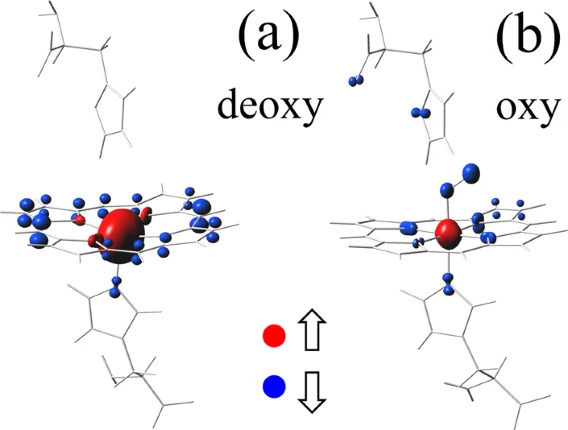
\includegraphics[width = 0.4\textwidth, height = 4.5cm]{assets/images/DeoxyHb_magnetic.jpg}
   \caption{Illustation of magnetic-moment density \textbf{M(r)} for the \textbf{(a)} \gls{HbR} and \textbf{(b)} \gls{HbO} heme clusters at \textit{T = 150K}. The magnitude of \textbf{M(r)} at an atomic site is proportional to the volume of the bubble at that site \cite{Mayda2020} Fig. 2 p.2).}
   \label{fig:HbMagnetic}
\end{wrapfigure}

% How BOLD manifests.
The \gls{BOLD} effect related to neural activity arises because of two distinct phenomena. The first is that when \gls{Hb}-the molecule in blood that carries oxygen-lose the oxygen to become \gls{HbR}, its magnetic properties change in a subtle way: \gls{HbR} is paramagnetic, and alters the magnetic susceptibility of blood, whereas \gls{HbO} and the surrounding tissue \ce{H2O} are diamagnetic \autoref{fig:HbMagnetic}. The difference in susceptibility between blood vessels and the surrounding tissue creates local magnetic field distortions that decrease the net \gls{MR} signal. In the brain, a typical \gls{OEF}-the fraction of \ce{O2} carried by an element of blood that is removed in passing through the capillary bed-is approximately 40\% and in a 3 T magnetic field this level of \gls{HbR} in the veins and capillaries is sufficient to reduce the \gls{MR} signal by about 10\% in the baseline state, compared to what it would be if no \gls{HbR} was present. 

The combination of the aforementioned with the biophysical phenomenon, that when a brain area is activated, the blood flow increases-via a process called the haemodynamic response-to a greater degree than the oxygen metabolic rate, produces a useful basis for an experimental signal aqcuisition technique. The second phenomenon leads to a reduction in the \gls{OEF}, a seemingly paradoxical scenario in which the venous blood is more oxygenated, despite the increase in oxygen metabolic rate, because the blood flow has increased to a greater extent. Taken together, these two phenomena produce the \gls{BOLD} effect, a local increase in the \gls{MR} signal due to a reduction in the \gls{OEF} during increased neural activity. \cite{Buxton2013}

% Misconception tackled.
A prevailing misconception is that \gls{BOLD} provides a direct measurement of neuronal oxygen consumption. However, this is generally not the case; classic positive \gls{BOLD} signals, seen in response to functional stimuli, represent a decrease in \gls{HbR} and thus an overoxygenation of the responding region \cite{Attwell2002}. These positive \gls{BOLD} responses correspond to a local, actively actuated, increase in blood flow and volume, which brings blood in sufficient excess to increase local oxygenation levels \cite{Raichle1998}. This response typically begins within about 500ms and peaks 3-5 seconds after stimulus onset \autoref{fig:BOLD}, even for short stimuli lasting less than 1 second, with more complex dynamics for prolonged stimuli.

\begin{figure}[H]
    \centering
    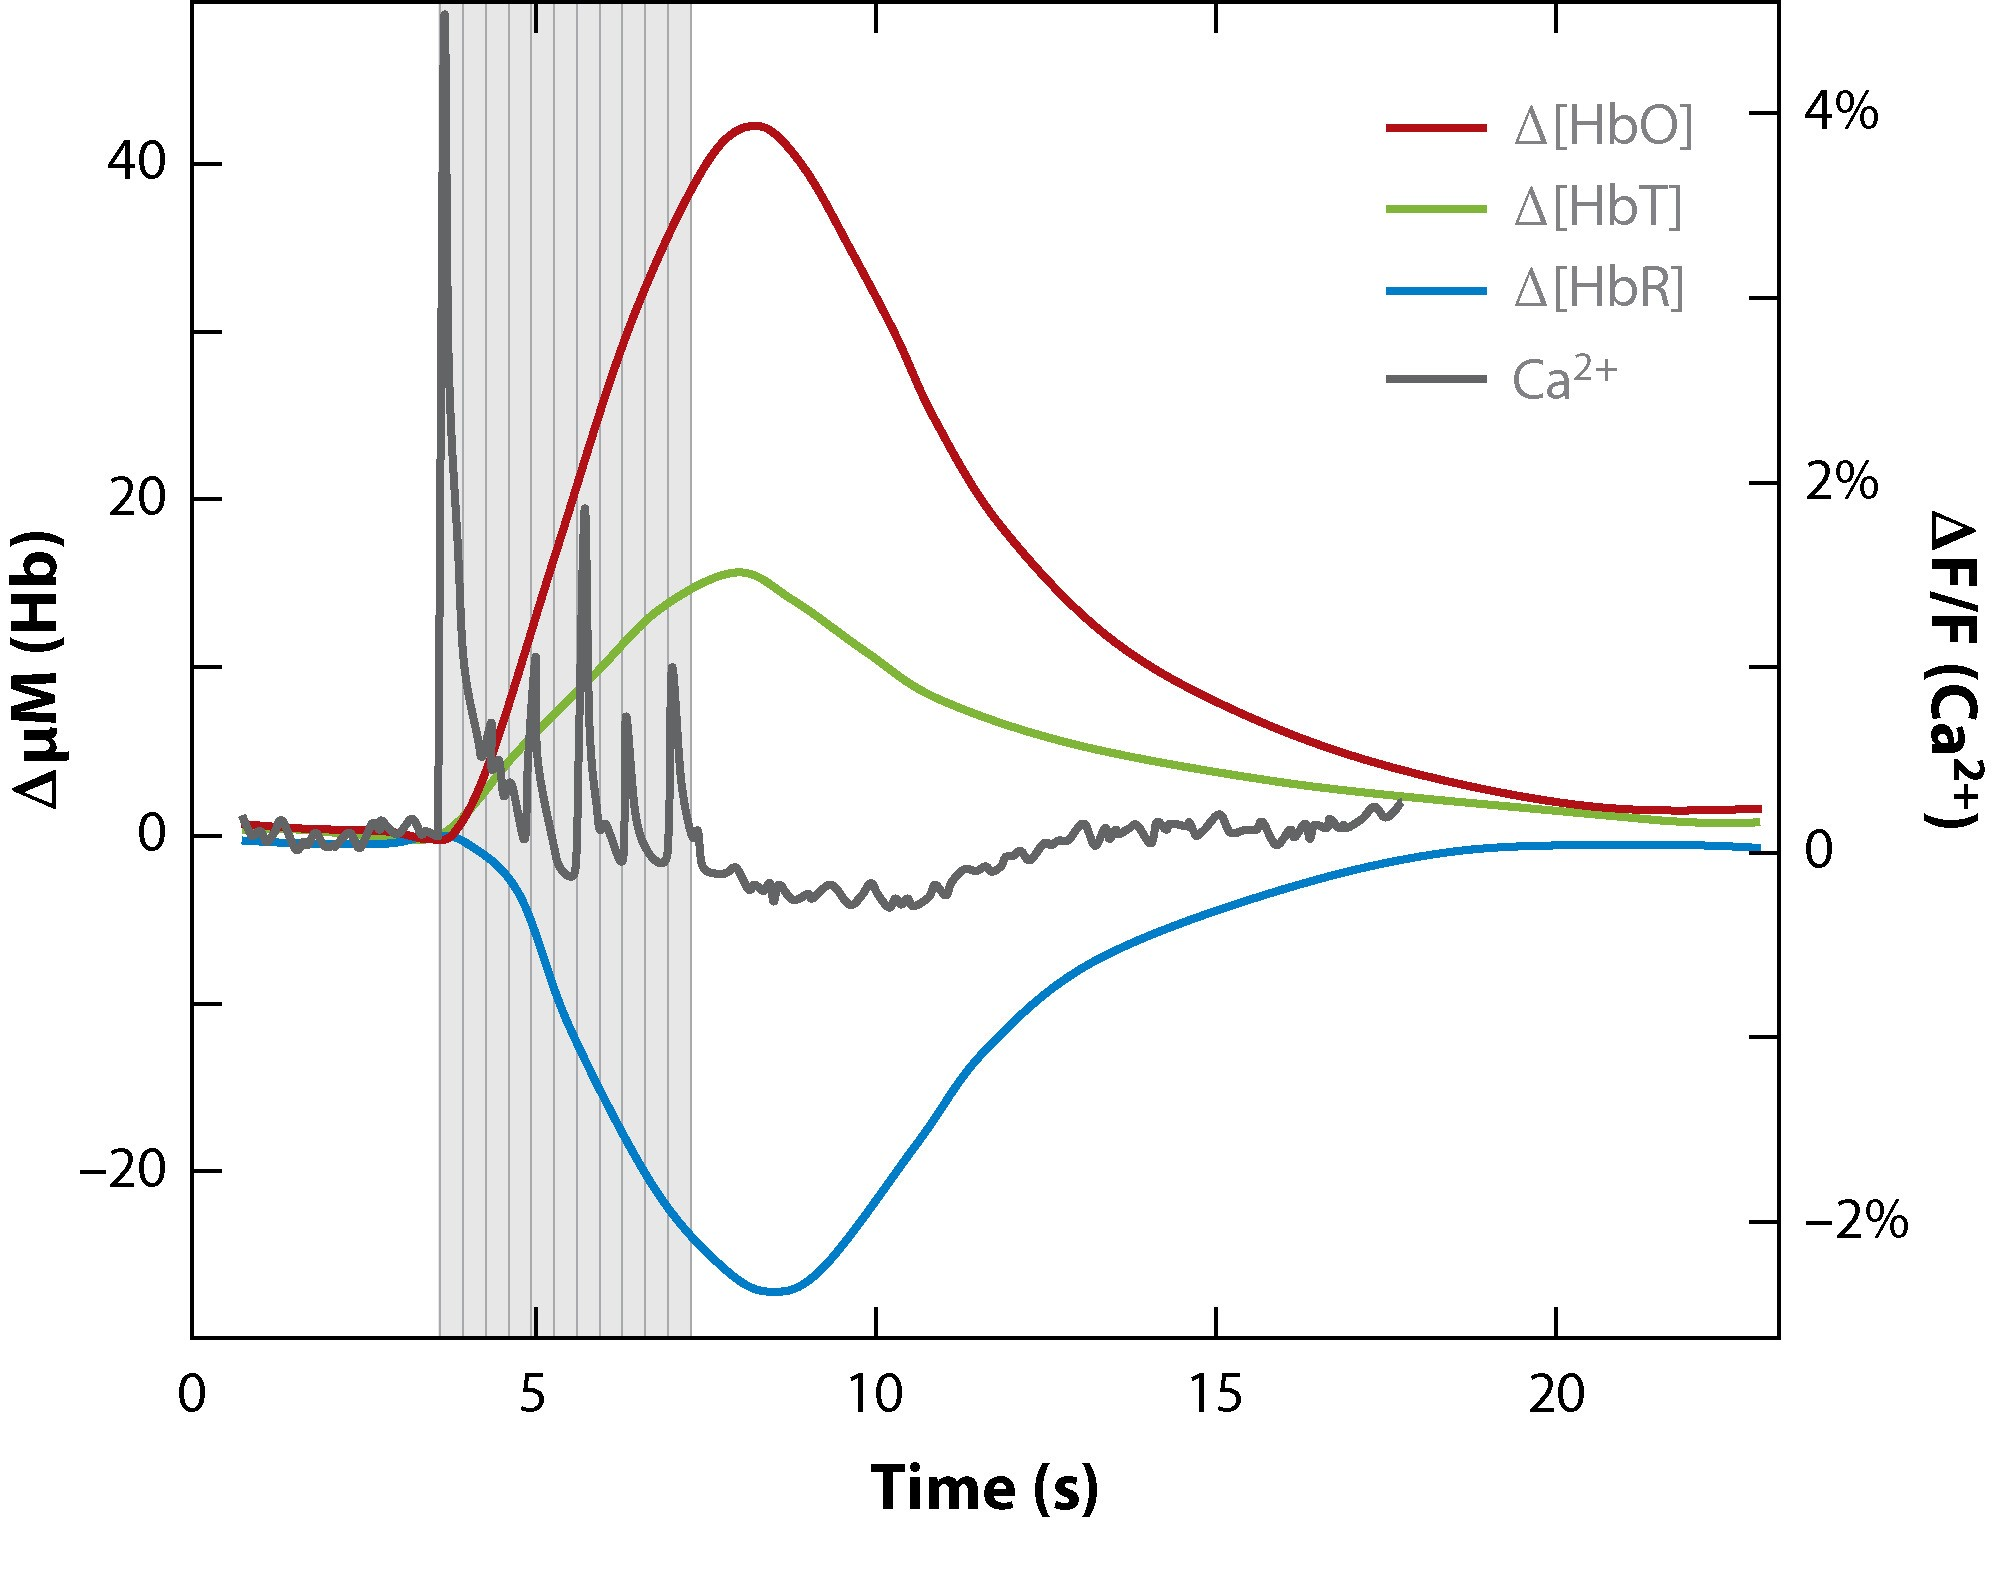
\includegraphics[width = 0.75\textwidth]{assets/images/Hb_flactuations_BOLD.jpg}
    \caption{Stimulus-evoked response in somatosensory cortex of rats. Noteably, there is a distinct increase in \gls{HbT} corresponding to vessel dilation and an increase in the number of red blood cells per unit volume of cortex, consistent with an increase in blood flow. \gls{HbO} increases while \gls{HbR} decreases, indicating a net overoxygenation of the region. The \gls{fMRI} \gls{BOLD} is sensitive to changes in \gls{HbR}, where stimulus-evoked "positive \gls{BOLD}" corresponds to the decrease in \gls{HbR} shown here \cite{Hillman2007} Fig. 2 p.4).}
    \label{fig:BOLD}
\end{figure}

% Broad finishing statements.
A range of cellular mechanisms, including astrocytes, pericytes, and interneurons, have been proposed to play a role in neurovascular coupling.\cite{Hillman2014}. For classical interpretation of \gls{BOLD} signals, it is assumed that neurovascular coupling is so robust that any increase in neuronal activity generates a proportional increase in local blood flow, irrespective of brain region, brain development, and pathological state \cite{Logothetis2010}.

\subsection{The HCP WM task experiment}

% Where the data was extracted from.
The data manipulated in this project has been obtained from the \gls{HCP} database, whose overarching purpose is to acquire and share data about the structural and functional connectivity of the human brain. One of the major categories of data in the \gls{HCP} refers to \gls{tfMRI} which assesses seven domains that sample the diversity of neural systems of interest, to a wide range of individuals in the field: 1) visual, motion, somatosensory, and motor systems; 2) category specific representations; 3) working memory or cognitive control systems; 4) language processing (semantic and phonological processing); 5) social cognition (Theory of Mind); 6) relational processing; and 7) emotion processing. \textbf{cite Barch2013, cite HCP somehow?}

\vspace{3cm}

\begin{wrapfigure}{r}{0.4\textwidth}
    \centering
    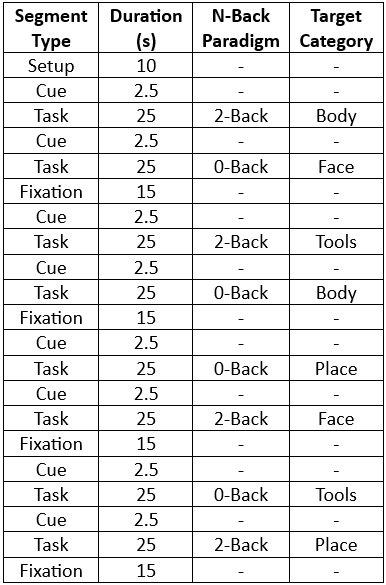
\includegraphics[width = 0.4\textwidth]{assets/images/WM_mat.png}
    \caption{Display of the exact sequece of events during the \gls{WM} task paradigm.}
    \label{fig:WM_mat}
\end{wrapfigure}

% How the experiment was conducted.
The domain which is presently being examined is that of \gls{WM} tasks which is combined with category specific representation tasks into the following, single task paradigm. Stimuli were projected onto a computer screen behind the subject's head within the imaging chamber. The screen was viewed by a mirror positioned approximately 8 cm above the subject's face. Participants were presented with blocks of trials that consisted of pictures of places, tools, faces and body parts (non-mutilated parts of bodies with no "nudity"). Within each run, the four different stimulus types were presented in seperate blocks. Also, within each run, half of the blocks use a 2-back \gls{WM} task and half use a 0-back \gls{WM} task (as a working memory comparison). A 2.5 second cue indicated the task type (and target for 0-back) at the start of the block. Each of the two runs contains eight task blocks (10 trials of 2.5 seconds each, for 25 seconds) and four fixation blocks (15 seconds). On each trial, the stimulis is presented for 2 seconds, followed by a 500ms \gls{ITI}. The procedure is showcased in order in \autoref{fig:WM_mat}.














%\subsection{T1 and T2,T2* times in fMRI?}

\pagebreak
\chapter{Category-Specific Data - MVPA}
\label{sec:cat_spec}

Add procedure explanation text here.
\pagebreak
\chapter{Software Architecture}
\label{sec:software}

Add pipeline explanation text here.
\pagebreak
\chapter{Classification Results}
\label{sec:classifier}

Add results text here.
\pagebreak
\chapter{Discussion \& Conclusions}
\label{sec:discussion}

Add conclusion text here.

% Helper sections
\newacronym{MVPA}{MVPA}{Multi-Variate Pattern Analysis}
\newacronym{UPA}{UPA}{Univariate Pattern Analysis}
\newacronym{SVM}{SVM}{Support Vector Machine}
\newacronym{ROI}{ROI}{Region of Interest}
\newacronym{ROIs}{ROIs}{Regions of Interest}
\newacronym{BOLD}{BOLD}{Blood-Oxygen-Level-Dependent}
\newacronym{HbR}{HbR}{deoxyhemoglobin}
\newacronym{HbT}{HbT}{total hemoglobin}
\newacronym{HbO}{HbO}{Oxyhemoglobin}
\newacronym{Hb}{Hb}{hemoglobin}
\newacronym{OEF}{OEF}{Oxygen Extraction Fraction}
\newacronym{HCP}{HCP}{Human Connectome Project}
\newacronym{WM}{WM}{Working Memory}
\newacronym{ITI}{ITI}{inter-task interval}
\newacronym{CSF}{CSF}{Cerebrospinal Fluid}
\newacronym{RF}{RF}{radio frequency}
\newacronym{CBF}{CBF}{Cerebral Blood Flow}
\newacronym{ASL}{ASL}{Arterial Spin Labeling}
\newacronym{USA}{USA}{United States of America}
\newacronym{T1w}{T1w}{T1-weighted}
\newacronym{T2w}{T2w}{T2-weighted}
\newacronym{MZ}{MZ}{monozygotic}
\newacronym{DZ}{DZ}{dizygotic}
\newacronym{IQ}{IQ}{intelligence quotient}
\newacronym{T-MEG}{T-MEG}{task-evoked MEG}
\newacronym{EV}{EV}{explanatory variable}
\newacronym{COPE}{COPE}{contrast of explanatory variables}
\newacronym{SVMs}{SVMs}{Support Vector Machines}
\newacronym{PCA}{PCA}{Principal Component Analysis}
\newacronym{ICA}{ICA}{Independent Component Analysis}
\newacronym{PDF}{PDF}{probability density function}
\newacronym{HRF}{HRF}{Hemodynamic Response Function}
\newacronym{GLM}{GLM}{General Linear Model}
\newacronym{NIfTI}{NIfTI}{Neuroimaging Informatics Technology Initiative}
\newacronym{LR}{LR}{Left to Right}
\newacronym{RL}{RL}{Right to Left}
\newacronym{FEAT}{FEAT}{FMRIB's Expert Analysis Tool}
\newacronym{3D MPRAGE}{3D MPRAGE}{three-dimensional magnetization-prepared rapid gradient-echo imaging}
\newacronym{FOV}{FOV}{Field of View}
\newacronym{BW}{BW}{Bandwidth}
\newacronym{ES}{ES}{Echo Spacing}

% fMRI Acronyms
\newacronym{r-fMRI}{r-fMRI}{resting-state fMRI}
\newacronym{t-fMRI}{t-fMRI}{task-evoked fMRI}
\newacronym{dMRI}{dMRI}{diffusion imaging}
\newacronym{fMRI}{fMRI}{Functional Magnetic Resonance Imaging}
\newacronym{MRI}{MRI}{Magnetic Resonance Imaging}
\newacronym{MR}{MR}{Magnetic Resonance}
\newacronym{NMR}{NMR}{Nuclear Magnetic Resonance}

% Imaging Techniques Acronyms
\newacronym{PET}{PET}{Positron Emission Tomography}
\newacronym{NIRS}{NIRS}{Near Infrared Spectroscopy}
\newacronym{MEG}{MEG}{Magnetoencephalogram}
\newacronym{EEG}{EEG}{Electroencephalography}

% Brain Anatomy Acronyms
\newacronym{LGB}{LGB}{Lateral Geniculate Body}
\newacronym{MT}{MT}{Middle Temporal visual area}
\newacronym{IT}{IT}{Inferior Temporal cortex}
\newacronym{FFA}{FFA}{Fusiform Face Area}
\newacronym{PPA}{PPA}{Parahippocampal Place Area}
\newacronym{LOC}{LOC}{Lateral Occipital Cortex}
\newacronym{EBA}{EBA}{Extrastriate Body Area}
\newacronym{FBA}{FBA}{Fusiform Body Area}
\newacronym{FG}{FG}{Fusiform Gyrus}
\newacronym{fSTS}{fSTS}{Superior Temporal Sulcus}
\newacronym{OFA}{OFA}{Occipital Face Area}
\newacronym{MOG}{MOG}{Middle Occipital Gyrus}
\newacronym{IOG}{IOG}{Inferior Occipital Gyrus}
\newacronym{LOS}{LOS}{Lateral Occipital Sulcus}

% Establishments Acronyms
\newacronym{WashU}{WashU}{Washington University}
\newacronym{UMinn}{UMinn}{University of Minnesota}
\newacronym{SLU}{SLU}{Saint Louis University}
\newacronym{NIH}{NIH}{National Institutes of Health}

% Glossary Entries
\newglossaryentry{V1}
{
	name = {V1},
	description = {Visual area V1, the striate cortex or primary visual cortex.\newline}
}

\newglossaryentry{V2}
{
	name = {V2},
	description = {Visual area V2, or secondary visual cortex, also called prestriate cortex.\newline}
}

\newglossaryentry{V3}
{
	name = {V3},
	description = {Visual area V3, which communicates directly with the respective dorsal and ventral subsystems of V2. It is less well-defined compared to other areas of the visual cortex.\newline}
}

\newglossaryentry{V4}
{
	name = {V4},
	description = {Visual area V4, a mid-tier cortical area in the ventral visual pathway.\newline}
}

\newglossaryentry{blob cells}
{
	name = {blob cells},
	description = {V1 cells that resemble kLGN neurons. They are monocular, color sensitive, characterized by small, concentric receptive fields and are found in clusters, hence the name.\newline}
}

\newglossaryentry{interblob cells}
{
	name = {interblob cells},
	description = {V1 cells, the majority of which are binocular, not color sensitive, characterized by elongated receptive fields, exhibit ocular dominance and orientation specificity, while they are found around the clusters of V1 blob cells.\newline}
}

\newglossaryentry{gyromagnetic ratio}
{
	name = {gyromagnetic ratio},
	description = {The gyromagnetic ratio, a constant specific to each different nucleus.\newline}
}

\newglossaryentry{TE}
{
	name = {Time of Echo},
	description = {The time between the delivery of the RF pulse and the receipt of the echo signal.\newline}
}

\newglossaryentry{TR}
{
	name = {TR},
	description = {The amount of time that passes between consecutive acquired brain volumes.\newline}
}

\newglossaryentry{flip angle}
{
	name = {flip angle},
	description = {The amount or rotation that net magnetization experiences during application of a RF pulse.\newline}
}

\newglossaryentry{connectomics}
{
	name = {connectomics},
	description = {The production and study of connectomes: comprehensive maps of connections within an organism's nervous system.\newline}
}

\newglossaryentry{2C}
{
	name = {2C},
	description = {The FEAT analysis that produced 2 chunks per subject, with a total of 40 chunks.\newline}
}

\newglossaryentry{4C}
{
	name = {4C},
	description = {The FEAT analysis that produced 4 chunks per subject, with a total of 80 chunks.\newline}
} % Input the glossary

% Print the glossary entries
\pagebreak
\printglossaries

% Print the references
\pagebreak
\printbibliography[heading=bibintoc]

\appendix
\input{Appendices/algorithms.tex}
\input{Appendices/snippets.tex}
\input{Appendices/code.tex}

\end{document}
